\chapter{Pocsékul}

\section{Egy Felépített Kép}

\keywords{felszínes benyomások, keserűség, hamis elvárások}

\noindent -- Helló, hogy érzed magad?\\
-- Pocsékul.

Egy meditációt gyakorló embernek nem ezt kellene mondania, ugye?
Pozitívan kellene válaszoljon, mint például, `Remekül érzem magam,
csodás napunk van!', vagy legalább, `Én megvagyok, és te hogy vagy?' Van
a fejünkben egy kép a `meditálóról', akitől elvárjuk, hogy bizonyos
módon viselkedjen és beszéljen, és bizonyos más viselkedés és beszéd nem
illik hozzá. Kérdezhetjük, `Ki ültette ezt a képet az \emph{én}
fejembe?'

A `jó meditáló' képe egy felületes benyomások alapján kialakult
észlelés, amiről engedtük magunkat, hogy valósnak tekintsük, mélyebb
vizsgálat nélkül. Gondolj arra, mikor megnyitottál egy meditációról
szóló cikket. (Miközben tovább olvasod a jelenlegit\ldots)

Egy fényképpel kezdődik, amin egy szerzetes vagy meditációs világi
tanító mosolyog, és az éberség pozitív hatásairól szóló leírással
folytatódik. Esetleg egy elvonuláson készült fényképeket és történeteket
is tartalmaz. Az emberek békés arccal ülnek a meditációs párnákon, míg
az ablakon keresztül áradó fény megvilágítja a Buddha szobrot. A cikkben
talán egy interjú részlet is olvasható arról, hogy valaki hogyan jutott
túl a belső küzdelmein. Egy meditációs tanító bátorító szavaival zárul,
vagy egy idézettel a Buddhától. VÉGE.

Még akit nem is érdekel túlságosan a meditáció is tudja milyen egy ilyen
cikk, mind láttunk már több tucatot. Nincs szükség forrás szöveget
megjelölnöm, az ebben a könyvben található fejezetek is például
szolgálhatnak.

Ezzel nem arra akarok utalni, hogy félre akarnának vezetni. A szerzők jó
szándékkal írnak. Bátorítani próbálnak minket, hogy haladjunk a
vizsgálódás ösvényén, és, hogy tegyünk erőfeszítést a gyakorlásunkban.
Ha a frusztrációkon túl nem látunk semmilyen nagyobb boldogságot, mi az
értelme az egésznek? Ha csak kín és szenvedés lenne várható, azt
segítség nélkül is létre tudjuk hozni.

\keywords{boldogság, állj félre a saját utadból, eltávolítani a sziklát a folyóból, vipasszana-glamúr}

A buddhizmus alapvetően optimista, és egyik központi témája a boldogság.
Saját hozzáállásunk jellemzően az, hogy keressük a boldogságot adó
dolgokat, vagy létre akarjuk hozni a boldogságunkhoz szükséges
körülményeket. Viszont nem biztos, hogy értjük a helyes hozzáállást, és
a boldogság keresésébe úgy bele tudunk gabalyodni, hogy egyre keserűbbek
leszünk, és úgy tűnik ez sosem lesz megvalósítható. Emiatt a
körülményeket, vagy saját képességünket tartjuk elégtelennek, de
valójában az a probléma, hogy dolgok természetes működését nem értjük,
és hozzáállásunk ezért vezet helytelen irányba.

A feladatunk, nem az, hogy a boldogságot keressük, hanem, hogy megértsük
a szenvedés keletkezésének okát, és ne hozzuk azt létre. Ennek
megértésén keresztül az elmében spontán megjelenik a boldogság.

Úgy gondolkodunk a dologról, mintha folyton egy szobrot faragnánk, amíg
az \emph{pont jó} nem lesz, de sosem vagyunk vele elégedettek. Úgy
gondoljuk ez a mi hibánk, és nem vesszük észre, hogy a szobrot alkotó
anyagok egyszerűen olyanok amilyenek. Az agyag, homok és kő, az marad
ami. A \emph{khandhák} csoportjai -- a forma, érzetek, észlelések,
mentális késztetések, és a tudatosság -- az marad ami. Abból ered a
küszködés, hogy mást várunk el tőlük.

Erőfeszítésre szükség van, de jobb metafora a bölcs gyakorlásra az
eltorlaszolt folyó képe: mint amikor kövek, sziklák akadályozzák a víz
folyását, és kavargó örvényeket hoznak létre. Hajlamosak vagyunk a
kavargó érzéseinkre összpontosítani, és miközben igyekszünk megállítani
az örvények forgását, egyre többet hozunk létre. Talán annyira lenne
csak szükség, hogy eltávolítsuk a sziklát, ami a folyást akadályozza:
azt, megragadjuk az egészet, mint `ez én vagyok'. Néha egyszerűen csak
félre kell állnunk a saját utunkból.

Ha megfigyeled a víz folyását egy folyó mederben, láthatod az
örvényeket, amik az akadályok mögött keletkeznek. Ezek oda-vissza
mozgása ismerősnek tűnhet (lásd \ref{fig-grasping-turbulence} ábra).
Mikor az elmében az `én vagyok' nézőpontja domináns, elkezdünk
oda-vissza csapódni az ellenkező álláspontok között. Magunkkal
vitatkozunk, mit tegyünk, mert `én szeretem az A-t', vagy `nem szeretem
a B-t', `X-et kellene csináljam', `nem kellene csináljam az Y-t'.

\enlargethispage*{\baselineskip}

Egyikkel sem vagyunk megelégedve, de megragadva tartunk egy énképet, az
elme benne ragad az extrém pontok közötti oda-vissza csapongásban. Az
egyik véglet a másikat hívja életre mint reakciót, az extrém pozíciókat
így könnyebben felvesszük, mint, hogy a helyzetet nyugodt fejjel
szemlélve külső nézőpontból értékeljük.

A tanítások valóban sokat említik a szenvedést, de az ilyen utasítások
arra alapulnak, hogy a szabadulás ettől a szenvedéstől lehetséges. A
Buddha világosan kifejtette, hogy az út gyümölcse őszinte boldogság, és
ha ezt gyakorolni nem lenne lehetséges, vagyis elhagyni a kártékony
gyökereket és fejleszteni a jótékonyakat, nem tanítaná ezt.\footnote{\href{https://suttacentral.net/an2.11-20/en/thanissaro}{AN
  2.19}, Jótékony Tényezők}

Ki ez a meditáló a fejünkben? Egy dolog biztos, aki az \emph{én
fejemben} van, mindig \emph{jobban tud meditálni} mint én. Amikor valaki
egy jó fotót készít rólunk, tudjuk hogy van ez: egy jó pillanat volt,
amikor rendezetten, akár glamúrosan is néztünk ki, de tudjuk, hogy öt
percen belül az ellenkezője is igaz lehet. Habár ez másokra is érvényes,
nem csak magunkra, valahogy nem emlékszünk erre amikor másokról készül
jó fotókat látunk.

Ezek afféle vipasszana-glamúr fotók -- kicsit hiú dolog, de szeretjük
látni őket. Jó illusztráció lesz belőlük egy cikkben, de emlékezzünk rá,
hogy ugyanazok az emberek máshogy néznek ki egy hétköznapi pillanatban.

\clearpage

\null\vfill

\begin{figure}[h]
\caption{Ragaszkodás és Kavargó Örvények az Elmében}\label{fig-grasping-turbulence}
\hspace*{-9mm}%
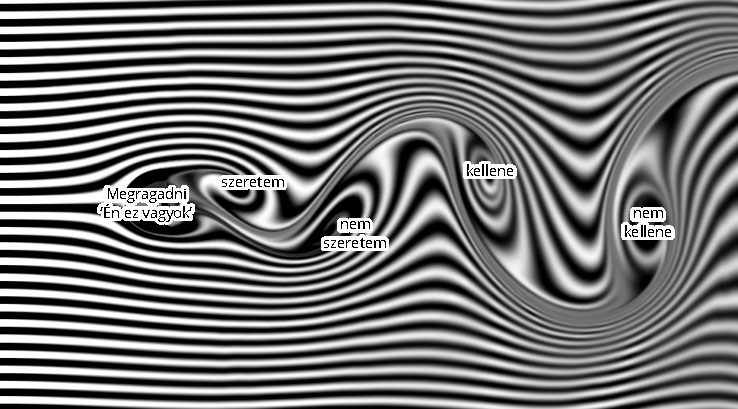
\includegraphics[width=\linewidth+18mm]{./manuscript/tex/diagrams/grasping-turbulence-hu.pdf}

\bigskip

{\small
Kavargó örvények egy akadályozott vízfolyamban.
Az örvények kialakulása hasonló ahhoz, ahogy az elmében az `Én vagyok' szemlélet megragadása következtében
az ember megragad az ellentétes pozíciók közötti oda-vissza csapongásban.
Folyadék szimuláció:
Amanda Ghassaei (\href{http://apps.amandaghassaei.com/VortexShedding/}{apps.amandaghassaei.com}).
\par}
\end{figure}

\vfill\null

\clearpage

\section{Szálak}

\keywords{a szutták mint irodalom}

\noindent A Buddha idejében az irodalom egyik formája a \emph{szutta}
volt, ami egy párbeszéd szálat jelent. A szutták tartalmazhatnak prózai
és verses szöveget is, azzal a szándékkal, hogy szavaláson keresztül
lehessen őket memorizálni. Egy jelentős eseményt követően a szerzetesek
közössége összeállított egy szuttát, ezzel formális alakba öntötték a
történetet és memorizálták azt. Erre a Buddha is szorgalmazta őket:

\begin{quote}
Így kell gyakorolnotok: `Jól oda fogunk figyelni, amikor a
tanítóbeszédeket recitálják, amelyek a Tathágata mélységes, mély
jelentésű, páratlan, az ürességre vonatkozó szavai. Hegyezni fogjuk a
fülünket, kitárjuk a szívünket a megismerésük felé. Úgy tekintünk rájuk,
mint amit megéri megragadni és a mesterévé válni.'
(\href{https://a-buddha-ujja.hu/sn-20.7/hu/fenyvesi-robert}{SN 20.7})
\end{quote}

Manapság a könyvek, cikkek, blog posztok töltenek be hasonló szerepet,
hogy tovább adják a megválogatott információt. Ezek a modern média
anyagok, mikor legjobb formájukat hozzák, a kánon szuttáit tartják maguk
előtt példaként. A korai idők szerzetesei ezeken a szálakon keresztül
juttatták el hozzánk üzenetüket, ez részévé válik az egymás közötti
párbeszédünknek azokkal, akikkel ma találkozunk, és írott munkáink
azokhoz szólnak a jövőben, akikkel mi már nem találkozunk.

\clearpage

\keywords{szociális hálók, szelekciós részrehajlás, Instagram Effektus}

A mai szociális hálókon az üzenet világos megértését torzítja az
úgynevezett `Instagram Effektus', ami egy szelekciós részrehajlás afelé,
hogy csak a legjobb és legpozitívabb oldalunkat mutassuk, és szűrjük ki
a negatívat, ami ennek ellenére éppen olyan valóságos és szükséges a
teljes megértéséhez.

Ez a befolyás nem elhanyagolható. Az orvosi tanulmányok már elkezdték
tárgyalni a depresszió és kényszeres viselkedés egy ide kapcsolódó
formáját, az ún. `Snapchat Diszmorfiát'.\footnote{\href{https://www.ncbi.nlm.nih.gov/pmc/articles/PMC5933578/}{Is
  ``Snapchat Dysmorphia'' a Real Issue? (ncbi.nlm.nih.gov)}} Ezekben az
esetekben az adott személy plasztikai sebészeti kezelést keres, hogy
külsője jobban hasonlítson az alkalmazásban látott mosolygó
fényképekhez.

Az app automatikus szűrői minden képet megváltoztatnak hogy vonzóbbá
tegyék, és ha az app ismételten úgy mutatja nekünk a saját testünket
mint egy szinte tökéletes kép, \emph{az} válik a mentális ön-képünkké,
és a szűretlen kép amit a tükörben látunk, helytelennek fog tűnni.

Egy hasonló Instagram Effektust vehetünk észre a meditációról szóló
cikkekben. A szerzőnek van egy mondandója, amihez a saját
tapasztalatából választ egy szeletet, hozzátéve a véleményeit és más
szerzők magyarázatát.

\enlargethispage*{\baselineskip}

A szerző írhat igazság-hűen és próbálhatja elkerülni az szelekciós
részrehajlást, de valamilyen szűrő mindig működésben van. Az írott szó
világa mindig egy felépített valóság. Viszont, mikor sikeresen eléri
célját, a jól megválasztott szavak nyomán ráismerünk a saját
tapasztalatunkra.

\clearpage

\keywords{mentális képeink mint példaképek}

A meditáló, aki a fejünkben él olyan, mint egy versben szereplő
karakter, vagy egy mítoszban szereplő hős. Hőseink bölcsebbek és
erősebbek nálunk, így amikor elveszettnek és gyengének érezzük magunkat,
hitet és tanácsot adnak nekünk. Az ő békéjük megrendíthetetlen, így
amikor pocsékul érezzük magunkat, képesek vagyunk kiállni azt és várni,
amíg a nehézség véget nem ér.

Az ilyen felépített mentális képek viszont nem mások, csak éppen azok,
nem tekinthetjük őket valódi személynek. Értékes források amikkel
önmagunknak irányt mutathatunk, a történetük leírása segít kitalálnunk
mit tegyünk, azáltal, hogy megmutatja hol vagyunk egy nagyobb kép
keretén belül.

Egy mentális kép szerepe nem az, hogy meghatározza \emph{mivé kellene
váljunk}. Amikor így viszonyulunk a képekhez és ideálokhoz,
önellentmondásokba keveredünk és elégtelennek érezzük magunkat, mert az
élet valós körülményei sokkal összetettebbek, képlékeny és változó
határai mozgásban vannak, nem úgy mint egy kép egy helyben álló,
leegyszerűsített valósága. A képek a magyarázat eszközei. A világra
tekintő \emph{látásmódot} nyújtanak, és példát a helyes cselekvés
irányára az adott fajta világban.

\clearpage

\section{Feltevések}

\keywords{az elme és a világ, a figyelem módja, tettek és hitek}

\noindent Felidézhetjük a Dhammapada verset, ami rámutat, hogy a
tapasztalatunk világa nem független tőlünk:

\begin{quote}
Az elme minden létállapot előtt jár, az elme vezeti őket, az elméből
származnak.

\emph{Manopubbaṅgamā dhammā, manoseṭṭhā, manomayā.}

\bigskip

\quoteRef{%

\href{https://suttacentral.net/dhp1-20/pli/ms}{Dhp 1}

}
\end{quote}

Ez azt jelenti, hogy képzeletbeli problémákat gyártunk magunknak?

Kezdhetjük a vizsgálatot ezzel a kérdéssel: `Képes az alany szenvedést
tapasztalni?' Élőlények szenvedhetnek, de egy kulturális fogalom, vagy
magunk által létrehozott történet nem tud szenvedni, még ha közben
\emph{mi} szenvedünk is. Megváltoztatja a hozzáállásunkat, ha az
aggodalmunk tárgya csak történetként létezik, mint egy intézmény,
nemzet, pénz, hírnév vagy egyéb társadalmi történet, és nem egy élő
lény.

Következő, egy gyors morális biztonsági teszt: `Egy bölcs ember vajon
dicsérné vagy kritizálná ezt?'

Folytatva, felszínre hozhatjuk a nézetünket: `Milyen feltevés hozza
létre ezt a feszültséget és nyomást? Mi ad jelentést nekem ahhoz, hogy
ezt tegyem? Mi az, ami nélkül ennek nem lenne jelentősége?'

Feltárhatjuk az ilyen tudattalan motivációkat azzal, hogy a jelen
tetteinket és választásainkat figyeljük. Amit most választunk megtenni,
kifejezi azt, amiben hiszünk, a korábban elfogadott feltevéseinket.

`Miért választom megtenni ezt, itt? Honnan ered ez a tett és hova
vezet?'

A mögöttes tényezők eredhetnek például a környezetünk által kondicionált
szokásokból. Talán sosem fejeztük ki gondolatban miért tesszük amit
teszünk, de azt éreztük, hogy \emph{az eredmények kifejeződnek rajtunk},
legyenek azok jók vagy rosszak.

A tettekkel kezdeni a vizsgálatot és úgy rákérdezni a gondolatokra egy
eredményes módszer. A belső csevegésünk közben mindenféle belső
ellentmondásokat mondunk magunknak, viszont a tetteink világos
referencia pontokat adnak.

\keywords{a legjobb hely a tanulásra, megfordítani a feltevéseket}

A hozzá kapcsolódó érzés lehet, hogy pocsék, de ha ezt jelzésként
kezeljük arra, hogy forduljunk az elme felé és vizsgáljuk azt, a
hozzáállásunk gyakorlatias és eredményes marad. `Ha már egyszer itt
vagyok, mit tanulhatok ebből?'

A feltevéseinkhez azon keresztül találunk hozzáférést, hogy felfedjük a
tudattalan motivációinkat. Ha egyszer már tisztán ki tudunk fejezni egy
feltevést, szabadságot nyerünk arra, hogy megfordítsuk, vagy elhagyjuk
azt.

Megkérdezhetjük, `Segít ebben a helyzetben, ha megfordítom a
feltevéseimet?' Talán az, hogy az ellenkező irányból tekintünk rá, éppen
az, ami a megbékéléshez kellett, vagy ahhoz, hogy felhagyjunk az üggyel
mint ami sosem létezett. Akárhogy is, már nem kényszerből cselekszünk:
szabadok vagyunk elengedni vagy \emph{választani} azt, hogy végig
folytatjuk.

\clearpage

\section{A Vihar Után}

\keywords{boldogság és sikerek}

\noindent A meditációs útmutatók azt mondják, `térj vissza a jelen
pillanathoz', de ez nem jelenti, hogy mindent szeretned kell amit ott
találsz. A lényeg, hogy ez az egyetlen hely ahol élni tudsz. Ha boldog
vagy, nem a jövőben vagy boldog, hanem a jelenben. Ha szenvedsz, nem
értheted meg a jövőben, csak a jelenben. Egyes helyzeteket semmilyen
agyalás és belső párbeszéd nem fog javítani, legjobb úgy nevezni ahogy
az van, és sztoikusan kivárni a vihart. Egy konfliktus valóban feszült,
elválni attól amit szeretünk szomorú, és életben lenni mindig a saját
halálunk tragédiájával végződik.

Hajlamosak vagyunk a sikert várni, és számítunk arra, hogy a kemény
munkánk a jövőben igazolódik. Vedd szemügyre óvatosan a siker
pillanatát, mit tapasztalsz? Lehet meglepetés, öröm, vidámság,
megkönnyebbülés, ami után minden visszatér a hétköznapi szintre. A
célról kiderül, hogy nem akkora megváltás, mint ahogy gondoltunk. Ha
intenzíven arra koncentráltunk, hogy oda jussunk, talán nem is
emlékszünk semmire az odavezető útról, és azon töprengünk hova tűnt a
sok idő. Olyan erősen leköt minket az, hogy eredményesek legyünk, hogy
elpazaroljuk a lehetőségünket arra, hogy éljünk.

\keywords{értékek, elfoglaltnak lenni, Hedonikus Taposómalom, kiégettség, megelégedettség}

\enlargethispage*{\baselineskip}

A halál felett szemlélődni egy igazmondó, noha kissé ijesztő, tükröt
tart az értékeink elé. `Ha ma este meghalok, boldogan emlékeznék arra,
hogy úgy élek, ahogy ma teszem?' Ez a kérdés többet fel tud kavarni a
psziché mélyből, mint szeretnénk. Emlékszem olyan időre, mikor a
reakcióm a `boldog' szóra kizárólag harag és önutálat volt.

A `Hedonikus Taposómalom' kifejezés leírja az adaptív folyamatot, amiben
minden új sikeres eredményt a pszichénk az új normának tekinti, és egyre
kisebb érzelmi hatást érzünk a céljaink elérése után. Mintha
taposómalomban járnánk, nem számít milyen erősen próbálja az ember
növelni a boldogság szintjét azzal, hogy a következő sikeres lépésre
törekszik, az ember továbbra is egy helyben marad. Az életünket azzal
töltjük, hogy az úton utazunk, nem a célállomásban nyaralunk. Ha
közelebbről megnézzük, még a célállomás puszta ötlete is szétfoszlik,
minta mikor berepülünk egy felhőbe. `Azt hittem ott látom, de most, hogy
ott vagyok, itt semmi sincs.'

Ennek ellenére úgy tűnik, továbbra is azt gondoljuk, hogy elfoglalni
magunkat, eredményesnek és hatékonynak lenni valahogy majd meg fog
minket menteni. Az egyik projekt befejeztével azt érezzük,
\emph{szükségünk van} egy másikra, mert elfoglaltnak lenni a létezés
egyetlen módja, amit ismerünk.

Az öreg bölcsek egyre ismétlik üzenetüket a megelégedettségről, de úgy
látszik el kell szenvedjük a kiégés fájdalmát, mielőtt felfogjuk mi az a
probléma amiről beszélnek.

Bertrand Russell felállítja a diagnózist: `A közeledő idegösszeroppanás
egyik tünete az a meggyőződés, hogy az ember saját munkája szörnyen
fontos.'\footnote{\href{https://www.goodreads.com/book/show/51783.The_Conquest_of_Happiness}{The
  Conquest of Happiness by Bertrand Russell}}

\clearpage
\figurepagelayout

\begin{figure}[h]
\caption{Eredmények és a Hedonikus Taposómalom}\label{fig-hedonic-treadmill}

\centering

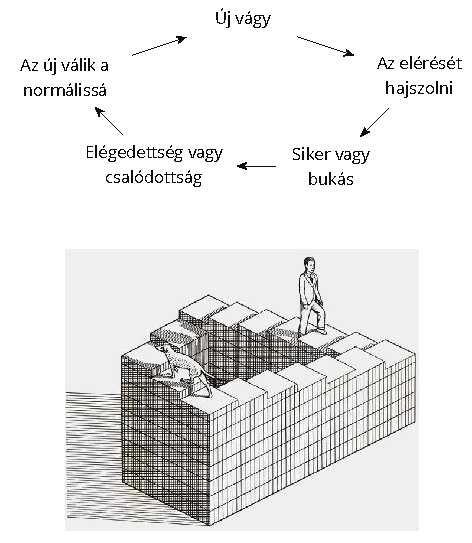
\includegraphics[width=90mm]{./manuscript/tex/diagrams/hedonic-treadmill-stairs-hu.pdf}

\bigskip

\begin{minipage}{0.85\linewidth}
\centering\footnotesize

A Hedonikus Taposómalom arra utal,
hogy hajlamosak vagyunk az új eredményeket egy új, \emph{normális} alapszintnek tekinteni,
és a boldogságunk szintje visszatér ugyanarra a szintre mint korábban.
Miután egy adott vágy beteljesül, a kondicionált szomj új állapotot keres.

\bigskip

A Penrose Lépcsőn lépkedő személy azt gondolja,
hogy egyre távolabbra és magasabbra jut.
A mi külső nézőpontunkból látjuk,
hogy csupán visszatér ugyanarra a szintre mint korábban.

\bigskip

Emlékezz a Szenvedés Keletkezésének Nemes Igazságának meghatározására:
`A folyton újraéledő, örömmel és szenvedéllyel járó, hol ebben, hol abban örömét lelő szomjúhozás, éspedig az élvezetek szomjúhozása, a ‘legyen’ szomjúhozása és a ‘ne legyen’ szomjúhozása.'
(\href{https://a-buddha-ujja.hu/sn-56.11/hu/a-pali-fordito-csoport}{SN~56.11})

\end{minipage}

\end{figure}

\clearpage
\normalpagelayout

Henry D. Thoreau kis fakunyhójában Walden Tó mellett azt írja: `Nehéz
dolog, ha déli hajcsárod van; még rosszabb, ha északi; de a legrosszabb
mind közül, amikor te vagy önmagad rabszolga hajcsára.'\footnote{\href{https://www.goodreads.com/book/show/16902.Walden}{Walden
  by Henry David Thoreau}}

Mi lenne, ha a \emph{szabad létezést} gyakorolnád, ahelyett, hogy
gyakorolsz azért, hogy \emph{szabaddá válj}? A fokozatos képzési
rendszer amit a Buddha kifejtett, -- miközben bátorít arra, hogy
szorgalmas erőfeszítést tegyünk a gyakorlásban -- a jelenbeli örömmel
kezdődik, ami megelégedettségből születik a morális- és érzéki
visszafogottságon keresztül.

\begin{quote}
{[}\ldots{]} Vigyáz az érzékeire, védi az elme tényezőit, visszafogja
azokat. Amikor birtokában van ez a nemes érzéki visszafogottság, nem
kifogásolható boldogságot tapasztal magában.

\bigskip

\quoteRef{%

\href{https://a-buddha-ujja.hu/mn-38/hu/a-pali-fordito-csoport}{MN 38},
A szomjúhozás kioltása

}
\end{quote}

\keywords{ön-ellenszenv, ön-kritika, tükrök labirintusa}

Könnyen túl-korrigáljuk a nyüzsgést, és átesünk a másik végletbe:
`Elegem van! Megszabadulok mindentől!' Ez ``logikusnak'' tűnhet, de az
ellenszenvtől hajtva tovább szenvedünk. Sokan vagyunk, akik könnyen
kritizáljuk magunkat, és szorgalmasan gyakoroljuk ezt, olyan
meggyőződéssel igyekszünk bebizonyítani a saját tévedésünket, mintha az
ön-ellenszenv egy erény lenne.

`Pocsékul érzem magam, aki \emph{valóban} tud meditálni sosem érezné így
magát. Biztos, hogy valamit rosszul csinálok.' Egy egész ön-azonosságot
fel lehet építeni ekörül, egy szüntelen belső monológot ami mindig
panaszokkal és ön-ellenszenvvel válaszol. Az ember évtizedeken át élhet
így, és ez válik az alap szintté, ami alapján felismerjük magunkat. `Ha
nem lennék ilyen mérges, nem is ismernék magamra.'

Olyan ez, mint beragadni egy tükrökből készült labirintusba: bárhova
nézel, csak magadat látod. A menekülés kulcsa, hogy találjunk egy
repedést a tükrökön és ismerjük fel a változást: ez a hajtott érzés, a
szorongás és harag motivációi amikről azt gondoltuk állandóak, valójában
folyton változnak -- szétesnek és újra formálódnak. A labirintust az
elme hozta létre, és amit létrehozott üres az éntől. Ez nem lehet az,
ami valójában mi vagyunk.

Kétségtelen, hogy tudunk meggyőző logikát találni az ön-meghiúsító
gondolatainkban, és érvelésünk a kritikus hozzáállásunk védelmében
teljesen észszerű is lehet! A pszichológusok azt mondják, hogy a
legnehezebben kezelhető betegeik azok, akik intelligensen védik és
indokolják saját rossz szokásaikat. Olyan okosak vagyunk, abszolút semmi
esély arra, hogy boldogok legyünk \ldots{} és be is tudjuk bizonyítani!
Emlékszel magadra, mikor az ilyen keserű filozófus szerepét játszottad?

Nem szükségszerűen jelent azonnali megkönnyebbülést, amikor
ön-vizsgálatunk felfedi előttünk az eddig keresett értékeink ürességét.
A harag, kétségbeesés\footnote{A Buddha a haraggal és kétségbeeséssel
  való küszködést ahhoz hasonlítja, mintha egy ösvényt követnénk, ami
  mellett mély szakadék tátong.
  (\href{https://www.accesstoinsight.org/tipitaka/sn/sn22/sn22.084.than.html}{SN
  22.84})} és szomorúság gyakran az első reakciók, és önutálattal
foglalkozó gondolatokat generálnak. Az elmét az elmével tisztítjuk meg:
Ezek az elme állapotok nem megbízhatóak, blokkolják az
intelligenciánkat, és azt ki akarja? Így elengedjük.

\keywords{türelmes kitartás, hála érzet, sietség nélkül}

A türelmes kitartás egy alábecsült erény, de gyakran nincs másra
szükségünk, csak hogy eszünkbe jusson várni: a kavargó elme állapotok
drámai mennydörgése ki fogja magát futni.

Amikor megjelenik a hála érzete, az olyan jel, mint a vihar utáni
szivárvány. A jótékony elme állapotokat kíséri, és intelligensen több
szögből is látjuk a helyzetet. Ez egy jó alap arra, hogy segítőkész
gondolatokat építsünk arról, hogy mit tegyünk. Néha az a legjobb, ha
egyszerűsítünk és elfordulunk bizonyos régi szokásoktól és értékektől.
Máskor, már megváltozott a nézetünk, és talán tovább folytatjuk amivel
eddig foglalkoztunk, de hátra hagyjuk a nagy sietséget. Azért
folytatjuk, hogy azt éljük, nem valamilyen emelkedett elmeállapotra
várunk a jövőben.

\begin{quote}
A múltat ne kergesd,\\
és ne álmodozz a jövőről.\\
Ami elmúlt az már mögöttünk van.\\
Ami eljön azt még nem értük el.

\bigskip

\quoteRef{%

\href{https://suttacentral.net/mn131}{MN 131}, Bhaddekaratta Sutta

}
\end{quote}

\clearpage

\section{Humor és Irónia}

\keywords{vélemények, változó nézőpontok, észrevenni a kellemeset}

\noindent A mogorva, sötét hangulatok olyanok, mintha magunk készítette
logikai csapdák lennének. Minél többet gondolkodunk róla, annál
mélyebbre süllyedünk bennük.

A humor és irónia éppen azért vicces, mert váratlan, furcsa szögből
mutatják a helyzetet. Ha a logikus út egyenesen előre el van zárva,
miért ne próbáljuk meg az oldalcsapást ahol a róka jár? Egy vicc nem
lenne vicces ha logikus és észszerű lenne. A humor és irónia, önmagunk
felé irányítva, jó barátnak bizonyulnak, amikor nem tudunk szabadulni a
saját gondolataink szenvedésétől.

Mitől lesz az öreg és bölcs ember \emph{bölcs}? Orvosi
tanulmányok\footnote{\href{https://www.researchgate.net/publication/258190619_Aging_irony_and_wisdom_On_the_narrative_psychology_of_later_life}{Aging,
  irony, and wisdom, William Randall (researchgate.net)}} megvizsgálták
az idős emberek különféle szemléletmódjait, és azt találták, hogy a
hajlamosság az önmaguk felé irányított humorra és iróniára (vagyis
amikor az ember képes nevetni önmagán) nagy segítséget jelent abban,
hogy szembenézzenek az öregedés jelentős kihívásaival, megőrizzék
szellemi egyensúlyukat és pozitív hozzáállásukat az élethez.

Egyik központi megfigyelésük az, hogy a humor és irónia fejleszti a
képességünket abban, hogy önmagunkat többféle nézőpontból is lássuk.
Egyidejűleg betölthetjük a pontos történész és a tréfáló komédiás
szerepét. Így többféle narrátori szögből is tudjuk látni az eseményeket,
és nem ragadunk be egyetlen történetbe. A narrátori keret amiben
magunkat látjuk, nyitott marad, és egy pozitív jövő irányába halad. A
létezésünk korlátai nem szükségszerűen jelentik a történet végét, és egy
jó nevetésért nem kell messzire menni: az élet abszurd sarkairól mindig
lehet egy jó viccet mondani.

Talán érzéketlen dolog valaki más rossz helyzetéről viccelődni, de ki
fog felháborodni a magadról szóló humoros megjegyzéseidről? Ha pocsékul
érzed magad, mit szólsz egy pocsék vicchez? Ez a menet olyan rossz, hogy
az már jó, és a jegyek ingyen vannak. `Mi vagyok én? Egy életre kelt
csontváz, egy bőrzsákban amire ruhákat aggatok, mesés frizurám alatt a
\emph{fontos véleményeim} logikáját bizonyítgatom.' Hol nincs ezen
nevetnivaló?

Gyakran mondjuk, hogy meditáció közben megfigyeljük a mentális
szokásainkat, de néha ezt egy kritikus elfogultságával gyakoroljuk:
megfigyeljük a \emph{rossz mentális szokásainkat}, és nem vesszük észre
a jókat. Annyira jók tudunk lenni abban, hogy figyelmen kívül hagyjuk a
kellemes elme állapotokat, hogy az ember őszintén elhiszi, hogy a
boldogság csak mások számára létezik. Amikor valami jó történik és
boldognak érzed magad, állj meg és vedd észre, `Na, ez milyen jó.' Ez
növeli a felfogó képességünket arra, hogy a jövőben is észre vegyük és
megtapasztaljuk a hasonló elme állapotokat. Ki fogja észre venni, ha te
nem?

\clearpage

\section{Elvárások}

\keywords{a Buddha szobrok szimbóluma, változó előrejelzések, eloldódás, elhagyás}

\noindent Az ember ránéz egy Buddha szoborra, és talán azt várja el
magától, hogy hasonlóan tökéletes testtartással meditáljon egyetlen
mozdulat nélkül, akár csak a Buddha. Ebben az esetben viszont
félreértettük a szobor üzenetét, ami belső tulajdonságokra mutat, nem
külső jelekre.

A Buddha szobrok nem a történelmi \emph{Sziddhárta Gótamát} ábrázolják,
aki az i.e. 5. században élt. Nem készült róla szobor az élete alatt. A
szuttákból tudjuk, hogy normális magasságú volt és szép küllemű, de arra
utasította a szerzeteseket, hogy ne a testi megjelenésével
foglalkozzanak, hanem a Dhammára, az elme igazságaira fordítsanak
figyelmet.

Azt tanította, hogy még ha egy szerzetes a csuhája sarkába kapaszkodva
követi, de nem látja a Dhammát, nem látja a Buddhát.\footnote{\href{https://suttacentral.net/iti92}{Iti
  92}, A Csuha Sarka} Az első Buddha szobrokat négy vagy ötszáz évvel a
halála után készítették a görögök, az afganisztáni Gandhára régióban. A
Buddha szobrok a felébredett elme bölcsességét és nyugalmát jelképezik,
az emberi formában kifejezve azt.

Gyönyörű rájuk nézni, de senki nem fog Buddha szoborrá válni, mint ahogy
nem válhatsz a tökéletes meditáló képévé sem, vagy a hőssé egy lírikus
költeményben. Tanácsot valóban adnak, de a tanács nem tud irányba
igazítani, ha mereven értelmezzük. Úgy kell alkalmaznunk, hogy
figyelembe vesszük a belső tapasztalatunkat és jelen helyzetünket. Így
visszatérünk a tudathoz, ami ráébred az igazságra és túllép az
akadályon. Az erény gyakorlása és a bizalom a nagy képességű tanítók
példájában erős alapot képez. Jót kívánhatunk magunknak, miközben el
tudjuk ismerni, hogy pocsékul érezzük magunkat, ha éppen olyan a
helyzet.

Az elvárások előrejelzik egy eredmény elvárt értékét, előre megbecslik a
helyzetünk kimenetelét. Eközben, minden tényező ami beszámít az
előrejelzésbe folyamatosan változik. Engednünk kell az előrejelzést is
változni, elvárásainknak a mentális tapasztalatunkról folyamatosan
változniuk kell aszerint, hol állunk éppen most. Az nem jelent
problémát, hogy elvárásaink vannak, de ha ragaszkodunk egy bizonyos
változathoz amit `az igazinak' hiszünk, éppen az válik akadállyá. Az
derül ki, hogy ha jövőbeli érzelmi állapotokba fektetjük a boldogságunk
alapját, az eredmény többnyire a csalódás.

Az \emph{ánápánaszati} légzés meditáció technikáját a Buddha tizenhat
lépésben tanította. Az első, hogy tudatosítjuk, a légzésünk hosszú-e
vagy rövid. Mi az utolsó lépés? Kíváncsian várhatjuk, `Mi lehet az a
fenséges elme állapot, amit végül magunkénak tudhatunk?' A légzésre
irányuló éberség meditáció a test, az érzések, és az elme állapotok
szemlélete után a természetes igazságok szemléletét tanítja, melynek
utolsó lépése:

\begin{quote}
`Az eloldódás fölött szemlélődve lélegzem be, így gyakorol. Az eloldódás
fölött szemlélődve lélegzem ki, így gyakorol.'

\bigskip

\quoteRef{%

\href{https://a-buddha-ujja.hu/mn-118/hu/farkas-pal}{MN 118},
Ānāpānasati Sutta

}
\end{quote}

A Nemes Nyolcrétű Ösvény gyakorlása nem a halmozásról szól, hanem az
értékeink átalakulásáról, a belátáson keresztül a körülmények
változásának tapasztalatába. Végül eloldódunk tőlük, elhagyjuk őket,
mintha letennénk egy terhet, nem cipeljük azt tovább. Ebbe minden
beletartozik, amit az `én és enyém' magába foglal: Meddig tudunk bármit
is megtartani?

\keywords{valódi gyakorlók, Imposztor Szindróma}

A vizsgálódás és fejlődés szélesebbre tárja a látóterünket, amiben az
ellentétek együtt tudnak létezni összetett kapcsolatokban. Az ellenkező
megközelítésben, a bíráló és ítélkező elme egy korlátozott körben mozog,
ami korlátozza a hatáskörünket. Az ilyen látásmód minden dolgot
rendszerezni akar szabályos, egymást kölcsönösen kizáró absztrakt
kategóriákba, ami bizalomvesztéshez és ártalomhoz vezet. Elkezdünk hitet
veszíteni, nem hisszük magunkról, hogy `valódi' gyakorlók vagyunk, és
egyúttal mások sem tűnnek hitelesnek. Az eredmény, hogy nem csak mi
magunk nem tudunk tanulni, de senkit sem tudunk elfogadni, hogy tanítson
minket. Ez a kétség megvakít és megbénít, úgy érezhetjük nem vagyunk
képesek semmit tenni. A probléma az, hogy az elvárásaink túl szűk
területre összpontosítanak.

Nem arról van szó, hogy ne lennének problémák és nehézségek. Azt
magyarázni magunknak, hogy a fájdalom nem fájdalmas, nem olyan
meditációs technika amit a Buddha tanított. Viszont nem kellene
feltételezzük, hogy olyannak kell lennünk mint a mitológiai ideáloknak.
A meditáció nem egy kapcsológomb, amivel irányítani tudjuk az elme
állapotokat, hanem a tudatosság fejlesztése, hogy az elme állapotok ne
irányítsanak minket.

\section{Érzelmek Kalibrálása}

\keywords{új érzelmeket tanulni, variáció a normális, csalódás, saññā és saṅkhāra}

\noindent Amikor egymásnak az érzelmekről beszélünk, gyakran úgy
magyarázzuk meg a működésüket mint egy `idegrendszeri áramkör', vagy az
agynak egy területe, ami bizonyos helyzetekben aktiválódik. Eszerint a
történet szerint, egyes agyterületek születésünktől fogva be vannak
kötve adott érzelmek kiváltására, és emiatt érzünk félelmet, szeretetet,
haragot vagy undort.

De akkor hogyan magyarázzuk, amikor valaki, akinek hiányzik az
\emph{amygdala} területe, mégis tapasztal félelmet? Az \emph{amygdalát}
jellemzően felelősnek tekintjük erre az érzelemre. Vagy mi a helyzet a
kifinomultabb kategóriákkal?

A japán `\emph{mono no aware}' jelentése a mulandóság miatti szomorúság
és ebben talált szépség érzése, a japánok vajon ilyen idegi áramkörrel
születnek? A leírás alapján talán magad felismered az érzést, ha láttál
japán filmeket, még ismerős is lehet, és most, egy szóbeli kifejezést
ráillesztve egyre könnyebben érezheted.

Más kultúrák a nyugati érzelmeket találják furcsának, mint például az
Utka eszkimók, akiknek nincs a `harag' koncepcióra közvetlen
megfelelőjük. Vagy a tahitiak, akiknek nincs `szomorúság'-nak megfelelő
képzetük.

\enlargethispage*{\baselineskip}

Az orvosi tanulmányok arról számolnak be, hogy semmilyen érzelemnek
nincs születéstől fogva beépített `áramköre'.\footnote{\href{https://www.goodreads.com/book/show/23719305-how-emotions-are-made}{How
  Emotions Are Made: The Secret Life of the Brain by Lisa Feldman
  Barrett}, Theory of Constructed Emotion} Nem az adott érzelem
alapvető, hanem a képességünk, hogy felismerjük a veszteség és nyereség
mintáit, hogy \emph{megtanuljunk érzelmi koncepciókat} más emberektől,
és felismerjük azokat egy új helyzetben a jövőben.

Egy adott helyzetben, az agy felismeri, hogy egy korábbi tapasztalat
\emph{egy ehhez hasonló kontextusban} nyereséggel járt vagy sem. Ez
idővel könnyebbé válik, ha megtanultunk hozzá társítani egy érzelmi
koncepciót, és ezzel spontán, automatikus érzéssé válik.

Egy érzelem kategória adott esete változó jellemű: a `félelem egy
tigristől' különbözik a `félelem egy vizsgától' érzéstől, melyek tanult,
adaptív előrejelzések. Csak bizonyos mértékben illeszkednek, mint ahogy
egy személyre ráilleszthető egy sztereotípia, de nincs olyan személy,
aki 100\%-os példája egy sztereotípia minden jellemzőjének.

Az agyunk kiértékeli a jelent a múlt alapján, és annak megfelelően, hogy
jó vagy rossz várható, egy választ érzünk a test különböző részein, és
ebből egy érzelem esetét alkotjuk a meglévő koncepcióink alapján.

\keywords{az érzelmek nem precíz mentális tárgyak, érzelmek tanulása, metta és sukha, mi a baj velem}

Az érzelmek klasszikus nézete szerint -- amihez hétköznapi
beszélgetésben vagyunk szokva -- az érzelmeket úgy kezeljük, mint
precízen mentális tárgyakat. Az elképzelés az, hogy egy érzelemnek
tisztán meghatározható jellemzői vannak, amiben két szellemileg
egészséges ember meg kell tudjon egyezni.

Viszont miközben az agyat működés közben tanulmányozták, nyilvánvalóvá
vált a tudósok számára, hogy ez semmiképpen nem lehet így. Ahogy egyre
több vizsgálatot végeztek, a bizonyíték folyton ellenkezett ezzel a
nézettel.

Amikor az emberek testi és pszichológiai teszteken mentek át, amiben
érzelmeiket vizsgálták, az eredmények nagyban különböztek az egyének
között. Nem volt semmilyen jól meghatározható, tisztán látható jelzés,
vagy `ujjlenyomat', ami beazonosíthatta volna bármelyik érzelmet.
Ehelyett, a \emph{változatosság volt a normális}, mind az egyének
érzelmi tapasztalataiban, azon érzelmek jelentésében és céljában, és az
ennek megfelelő testi reakciókban.

A tudósok azt találták, hogy a test és az agy \emph{megtanulja} az
érzelmi kategóriákat az észlelések kondicionáló folyamatán keresztül.
Saját kultúránkból, más emberektől akikkel együtt élünk (társadalmilag
kondicionált érzelmek); biológiai szükségleteinkből (testileg
kondicionált \textasciitilde); vagy személyes élményeink alapján, mint a
régi szokások, jelentős események és emlékeink.

Ez ahhoz is kapcsolódik, hogy egy adott személy nem mindig érti, vagy
talán fel sem ismeri egy másik ember érzelmeit. Gondolj például a
kultúr-sokkra, amikor egy távoli országba utazol: egy érzelemnek, mint a
`szeretet', változatos kifejezési formái vannak, olyan kontextusai és
mögöttes feltevései, amik nem voltak részei a saját érzelmi
kategóriánknak a `szeretetre'. Eltarthat egy ideig, amíg hozzá szokunk
az új jelekhez és jelentésekhez, ráérzünk az árnyalt különbségekre, és
megbízhatóan fel tudjuk ismerni a jeleket másokon.

Kérdezd meg magadtól, honnan tudod, hogy egy adott érzelmet érzel, mint
a \emph{metta} (szerető kedvesség) vagy \emph{sukha} (boldogság)? A
modell, amit érzéseink megértésére használunk, befolyásolja mit várunk,
hogy meditációs gyakorlásunk alatt történjen. Ha az érzelmekre úgy
tekintünk, mint határozott dolgokra, mintha külső tárgyak lennének amit
reprodukálnunk kell, vagy hozzá kell férjünk, könnyen úgy fogjuk érezni,
`ez nem az, nem tudom mi a baj velem.'

Mivel a \emph{változatosság a normális}, saját tapasztalatunk
valószínűleg különbözni fog másokétól. Az egyéni meditációs
tapasztalatok olyan változatosak, mint az egyének maguk. Egy érzelem
adott esetétől várható, hogy eltér az általános fogalomtól. Fontos, hogy
arra támaszkodjunk, hogy ismerjük a \emph{saját} elménket és
érzéseinket, ahelyett, hogy külső leírásokat próbálunk reprodukálni.

A szabadságunk arra is kiterjed, hogy megtanuljunk és létrehozzunk olyan
érzelmeket, amikről korábban nem is hallottunk. Az éberségre támaszkodva
észleljük a tapasztalatunkat, önmagunkat képezzük a koncepcióra, és
megteremtjük a feltételeket az érzelem megjelenésére.

Az Öt Khandha terminológiájával úgy mondhatnánk, hogy az észlelések
(\emph{saññā}) és mentális késztetések (\emph{saṅkhāra}) egymást
befolyásolva megalapozzák a tapasztalat mintáit, amit megtanulunk
beazonosítani mint egy szélesebb, absztrakt érzelmi kategória jelenbeli
esetét.

A külső leírások olvasásával kezdjük, és ezt belső tapasztalattá
alakítjuk át a vizsgálódáson és mindennapos tetteinken keresztül.
Megismerni a tapasztalatunkat referencia pontot ad. Idővel, az új
tapasztalatok ismerőssé válnak és erőlködés nélkül megjelennek.

\keywords{az érzelmek mint előrejelzések, kultúr-sokk, elvárások igazítása}

Az agy folyamatosan kapja a jeleket az idegrendszertől, és az alapján,
hogy mit tanult a múltbeli tapasztalatok alapján, próbálja megítélni,
hogy vajon a jelen helyzet energia bevitelt vagy energia kiadást fog
jelenteni a test számára.

Az agy válaszként felkészíti a tested, mint például növeli vagy
csökkenti a szív ritmust, beindítja vagy megállítja bizonyos hormonok
termelését. Ezt a testi reakciót tapasztaljuk, és ha korábban
megtanultunk egy érzelem kategóriát aminek ez megfelel, az adott érzelem
egy változatát érezzük: a veszélytől való félelem, az azonnal várható
jutalom izgalma, vagy a szárnyaló boldogság.

Ez magyarázza a kultúr-sokkot: ha más kultúrában nőttél fel, más érzelmi
kategóriákat tanultál, és amikor egy távoli országba utazol,
ismeretlennek hathat számodra az ott élő emberek érzelmi világa.

Hajlamosak vagyunk azt hinni, hogy a tapasztalatunk olyan, mint a
látvány amikor kinézünk az ablakon. Az ember `ránéz a tapasztalatára',
és látja mi történik.

Gyorsan kiderül, hogy amit látunk sokkal hiányosabb, mint gondoljuk, ha
meggondoljuk hogyan működnek az érzékek és az idegrendszer. Az agy nem
kap túl sok információt, amivel dolgoznia kell, és néhány egyszerű
jelből meg kell tippelnie, milyen lehet a gazdag világ, ami rajta kívül
van.

Az agy nem lát túl sokat: ott kuksol a koponyában, ami olyan, mint egy
sötét doboz. Testi folyadékok, vegyületek és idegrendszeri jelek
üzeneteket továbbítanak ebbe a dobozba. Az üzenetek a test már
rendszereitől erednek, amik maguk is zajosak és néha egymásnak
ellentmondanak. Ebből a kavalkádból az agynak létre kell hoznia az
észlelt képet arról, hogy hol vagyunk, megtippelnie mi történik velünk,
megjósolnia valószínűleg mi fog történni a következő pár percben, és
produkálnia kell egy választ, ami remélhetőleg segít bennünket a
túlélésben, vagy akár még boldogsághoz is vezethet. Ezt mind egy sötét
dobozon belülről kell véghez vigye, néhány zajos és korlátolt jelzés
alapján.

\clearpage

Mi vagyok tehát? Egy életre kelt csontváz, a fejem pedig egy sötét
doboz? Ez sok zavarodottságot megmagyaráz. Csoda-e, hogy az elvárásaim
egy kicsit félrecsúsznak, és folyamatos igazgatásra van szükségük? Amit
valóságként tapasztalok, egy folyamatban lévő találgatás eredménye, ami
másodpercenként változik.

`A boldogság egyenlő: valóság mínusz elvárások' -- Tom Magliozzi mondása
szerint. Manapság az elvárásaink olyan magasak. Frissítéseket kapunk a
szociális média appoktól, web cikkeket olvasunk, és minden alkalommal
befolyásolják a nézetünket arról, hogy vagyunk és hogy áll a világ
körülöttünk. Tökéletes, elhatározott, felháborító képeket mutatnak
nekünk más emberekről. Mivel nem találkozunk ezekkel az emberekkel
szemtől-szembe, nem látjuk az életük valóságos hátterét, és ez
felnagyítja az elvárásainkat. Ez újra és újra arra képezi az agyat, hogy
ezeket a mesterségesen létrehozott benyomásokat várja el, mint egy
túlhajtott elvárás-gép. Észre sem is vesszük ezt a torzított
ön-kondicionálást, de csalódottak és kimerültek vagyunk, ami szüntelen
elégedetlenséghez vezet.

\keywords{egyszerűség, állandótlanság, ön-vizsgálat, értékek}

Viszont megvan a képességünk, hogy kalibráljuk az `elvárás gépet', a
tudatos vizsgálódás és megfontolás kiegyensúlyozó hatásával. `Mi a
legfontosabb a mai nap? Mire van szükségem ehhez az egy naphoz?' Ha
leegyszerűsíted a választ a lényegre, nem olyan sok. Étel, ruha,
szállás, gyógyszer, támogató szellemű társak és talán valami tennivaló
egy érdemes cél irányába.

Az átlagos nap valószínű, hogy kuszább ennél, és nem igazodik az ilyen
absztrakt, tiszta egyszerűséghez, de ez arra szolgál, hogy felismerjük
az alap szintet. Ha az egyszerű is elegendő, akkor nem jelent problémát,
hogy többet is tudunk tenni, vagy több mindenhez is hozzáférünk, amíg a
megelégedettség marad az alap szintünk. Nem a törekvés a probléma, de az
elvárások felnagyítása blokkolja annak megvalósítását.

Az elvárások szükségesek ahhoz, hogy egy adott irányt kövessünk a
világban, de ha nem értjük őket, akadályokká válnak a szívben. Az
elvárások és érzelmek természete az, hogy megjelenjenek, és ide-oda
fordulva változzanak. Hagyd, hogy tovább ússzanak, mint falevelek a
csónak mellett. A rosszak nem olyan rosszak, a jók nem olyan biztosak.
Ismerve a változó természetüket, nem vesszük őket olyan komolyan, és nem
akadunk fenn bennük, mint ahogy egy csónaknak sem kellene fenn akadnia
holmi leveleken.

\begin{quote}
Legyen kellemes vagy fájdalmas,\\
a semlegessel együtt,\\
Akár belső, akár külső,\\
Bármilyen érzés ami van:\\
Megismeri, `Ez is szenvedésnek van kitéve,\\
megtévesztő és szétbomló',\\
Újra és újra érintve őket,\\
elmúlásukat szemlélve,\\
a szenvedélytől megszabadul.

\bigskip

\quoteRef{%

\href{https://suttacentral.net/sn36.2/pli/ms}{SN 36.2}, Sukha Sutta

}
\end{quote}

\clearpage

\section{Virágzó Élet}

\keywords{a boldogság jelentései, eredmények, egyszerre egy napot gyakorolni, halál, megelégedettésg}

\noindent A modern nyugati kultúránk a boldogságot gyakran úgy mutatja
be, mint egy meghatározott érzés, vagy egy bizonyos élethelyzet ahova el
kellene érkezzünk. Kultúránkat átadjuk egymásnak a közös párbeszéden át.
A boldogságról olyan módon beszélünk, mint egy eredményről, egy
eseményről a jövőben, vagy mint egy bizonyos létállapotról. Úgy tűnik,
ez egy nemrég kialakult szokásunk, és nem egy kifejezetten jótékony
hatású.

Hagyomány szerint az ókori görögökre úgy tekintünk, mint az egyik
legnagyobb befolyású társadalomra a nyugati értékeink kialakulásában.
Arisztotelész (i.e. 384-322) az egyik ilyen nagy befolyású gondolkodó,
és a mai napig olvassuk és visszautalunk a fennmaradt írásaira. Ezekben
a szövegekben részletesen vizsgálja a boldogság kérdését.\footnote{\href{https://plato.stanford.edu/entries/aristotle-ethics/}{Aristotle's
  Ethics (plato.stanford.edu)}} Láthatóan erősen foglalkoztatta, hogy mi
a boldogság, hogyan élhet az ember boldogan, viszont tőlünk eltérően,
nem úgy tekintett rá, mint egy adott eredményre vagy életkörülményre.

\enlargethispage*{\baselineskip}

A görög szó, amivel a boldogságra utal az \emph{eudaimonia}, fordításban
`emberi jólét, virágzó élet.' Úgy látta ezt megjelenni, mint egy
folyamatosan aktív folyamatot, amit nap mint nap gyakorlunk, nem pedig
egy eredményt, amit egyszer majd a jövőben elérünk. A boldogság
gyakorlását a morális erényekre alapozza, és az ember saját életére
vonatkozó valósághű szemléletre, ami a születéssel, a növekedés éveivel,
és az öregkorral együtt magába foglalja az ember saját halálának
tragédiáját.

Az erény és halandóság ilyen közvetlen szemlélete sorba rendezi a
dolgokat: egy tágas nézőpontot ad, amiben a boldogság a jótékony
szellemi tényezők alapjára épül, de önmagunkon túl kell néznünk ahhoz,
hogy hosszú távú jelentést adjunk annak.

Az elvárásainkat így képezve, a boldogság gyakorlata minden nap teljes
egész. Megtanulunk a nehézséggel együtt lenni, ha éppen úgy áll a
helyzet, és legjobb képességünket erényesen alkalmazva minden nap végén
megnyugvással tekinthetünk vissza.

A pszichológia `boldogság kutatás' területén Daniel Kahneman és csapata
interjúkat végeztek, amikben arra kérték az embereket, hogy idézzék fel
az előző napi eseményeket, és később válaszoljanak az erről szóló
kérdésekre.\footnote{\href{https://www.goodreads.com/book/show/11468377-thinking-fast-and-slow}{Thinking,
  Fast and Slow by Daniel Kahneman}, Day Reconstruction Method} A
kiértékelés megerősítette, hogy a figyelem és az ismétlődő gondolatok a
domináns tényezők abban, hogy valaki boldognak vagy depressziósnak érzi
magát. Miközben a jelentkezők különböző hétköznapi helyzeteken mentek
át, nem az határozta meg azt, hogy miként érezték magukat, hogy hol
voltak és mit csináltak, hanem, hogy miről gondolkodtak éppen akkor.

\keywords{megbánás a halálos ágyon, az élet mint idő egység, a szükségletek hierarchiája, ön-megvalósítás, ön-meghaladás}

\enlargethispage*{\baselineskip}

Az viszont meglepetésként érte őket, hogy amikor az emberek arról
beszéltek milyen napjuk volt, nem a boldogságról beszéltek mint egy jó
érzésről, sokkal inkább arról, hogy milyen társasági élményeik voltak,
barátokkal és rokonokkal, kivel találkoztak és mit csináltak együtt, és,
hogy elégedettnek érezték-e magukat az életükkel, vagy sem.

Ez érthető, ha megvizsgáljuk saját tapasztalatunkat: a szemlélet, a
keret amin keresztül a világot látjuk adja meg a tájékozódási
pontjainkat, miközben a keret tartalma folyamatosan változik. Az éhes
ember a világot az ételszerzés szemszögéből látja. Aki célratörő
hangulatban van arra összpontosít, hogy `mire vagyok képes', és `milyen
jó vagyok.' Aki eltöpreng milyen korlátozott idejű a személyes létezése,
hajlamos olyan értékek felé fordulni, amik önmagán túlmutatnak.
Ahelyett, hogy az `én' által létrehozott tapasztalatok foglalkoztatnák,
az ember az időtlen jellemzők felé fordul, amik itt és most láthatóak.

Számomra felfedezés volt, mikor egy interjút hallgattam,\footnote{\href{https://www.samharris.org/podcasts/making-sense-episodes/209-a-good-life}{A
  Good Life: A Conversation with Scott Barry Kaufman}} és hallottam a
pszichológusokat arról beszélni, hogy egy új elemet adtak hozzá Abraham
Maslow ú.n. szükségletek hierarchiájához. Ezt rendszerint egy
piramisként ábrázolják, ami az alsó szinten az étel- és víz
szükségletével kezdődik, majd az ön-megvalósítással végződik, amit a
csúcsra emel. Ez a boldogságról egy meglehetősen én-központú
gondolkodási módnak tűnt.

\enlargethispage*{\baselineskip}

A pszichológusok nemrég újra elővették Maslow későbbi
írásait,\footnote{\href{https://bigthink.com/neuropsych/maslow-self-transcendence/}{Maslow's
  forgotten pinnacle: Self-transcendence (bigthink.com)}} és azt
találták, hogy az élete végéhez közeledve, konfliktusban érezte magát
saját rendszerével az értékek hierarchiájáról: hamarosan meg fog halni,
szükségleteinek alapvető részei (mint a túlélés) hiányoznak, tehát
nyomorúságosan kellene érezze magát, de ehelyett, felszabadultságot és
olyan boldog állapotokat érzett, amit `csúcs-élményeknek' nevezett:

\begin{quote}
Az érzések határtalan horizontja nyílik meg a szem előtt; az érzés, hogy
erőteljesebb, és egyúttal gyámoltalanabb vagy mint korábban bármikor; a
hatalmas eksztázis, csodálkozás és révület érzése; elveszíteni hol vagy
időben és térben; és végül -- a meggyőződés, hogy valami kifejezetten
fontos és értékes történt, mely élmény nyomán az ember részben átalakult
és megerősödött, kihatással a hétköznapi életére is.
\end{quote}

Maslow hozzácsatolt még egy szintet a szükségek hierarchiájához, az
ön-megvalósítás felett: \emph{az ön-meghaladást}. Ennek példái: nem
ragaszkodni a tökéletességhez, nem tartani mereven saját véleményünket,
feladni a bizonyosság szükségét, feladni a saját múltunkhoz való
ragaszkodást, és elengedni a haláltól való félelmet.

Az `ön-meghaladás' úgy hangzik, mint ami egy Buddhának való, de mivel
szenvedünk a ragaszkodásainktól a különféle dolgokhoz, kiderül, hogy ez
mindannyiunknak számára egy alapvető \emph{szükséglet}.

\enlargethispage*{\baselineskip}

A ragaszkodás ahhoz, amiről azt gondoljuk mi vagyunk, hozza létre éppen
azokat a korlátokat, amikkel küszködünk. Egyre szélesebb körű horizontot
akarunk látni, de visszatart minket, hogy egy ön-azonosságba
kapaszkodunk. Amikor arról az azonosságról kiderül, hogy egy üres tér,
sürgős segítségre van szükségünk. Gondolj a mindennapos küzdelmekre:
konfliktusba kerülünk a véleményünk miatt, feszültek vagyunk a
képességeink hiánya miatt, idegesek vagyunk a váratlan változásoktól,
siratjuk a múlt tragédiáit. Szükséges egy ön-meghaladó szemlélet, hogy
túltegyük magunkat magunkon.

\clearpage
\figurepagelayout

\begin{figure}[h]
\caption{Szükségletek Hierarchiája, Ön-meghaladó Értékek}\label{fig-self-transcendental}
\bigskip
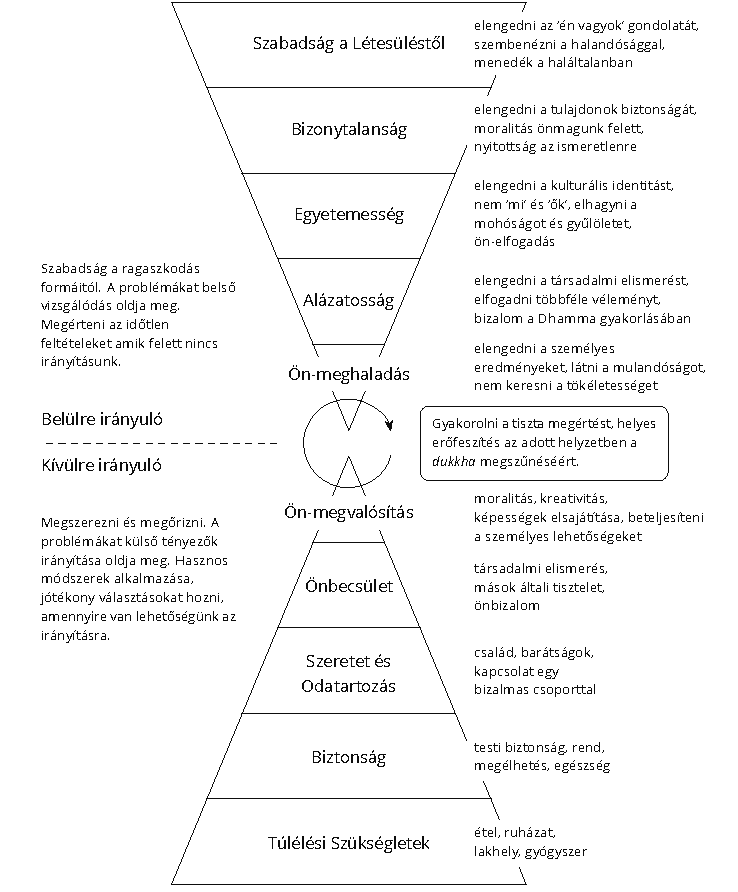
\includegraphics[width=\linewidth]{./manuscript/tex/diagrams/self-transcendental-values-hu.pdf}
\end{figure}

\clearpage
\normalpagelayout

Mégis, számon tartjuk hogy állnak a dolgaink az életben, nem igaz? A
jótékony tényezők a támogató alapot jelentik. Ez az a hely és idő ahol
élünk, nem egy másik: \emph{memento vivere}, emlékezz, hogy élj. Tudjuk
magunkról, hogy az erőfeszítéseink összhangban állnak a központi
értékeinkkel vagy sem, még akkor is, ha elterelik a figyelmünket olyan
dolgok, amiken nem terveztünk olyan sok időt tölteni.

Emlékszem engem mennyire felrázott, amikor azt olvastam egy ápolónő
beszámolójában,\footnote{\href{https://bronnieware.com/blog/regrets-of-the-dying/}{Regrets
  of the Dying (bronnieware.com)}} hogy a halálos ágyon mondott
leggyakoribb megbánások közé tartozik a túl sok munkával töltött idő, és
elveszíteni a kapcsolatot a régi barátokkal. Az élet egy idő egység,
aminek kezdete és vége van, és ennek megfelelően kell azt kezeljük.

\keywords{\emph{memento mori}, \emph{memento vivere}, \emph{amor fati}, \emph{saṃvega}, \emph{pasāda}}

Ha az elmét egy kényelmes tompaságban elmeríteni azt jelenti, hogy
`benyugtatózzuk magunkat a triviális dolgokkal', akkor emlékezni a
halálra (\emph{memento mori}) egy adag anti-nyugtatót jelent. Mivel az
idő korlátozott, emlékszünk a sürgetésre, hogy éljünk (\emph{memento
vivere}), és tegyük meg amit kell mielőtt túl késő. Ez motivációt ad,
hogy megtaláljuk a bátorságot arra, hogy igazak legyünk önmagunkhoz, és
forduljunk a helyzet felé amiben élünk (\emph{amor fati}), ne várjuk
valamilyen képzeletbeli helyre és időre a jövőben. A buddhista
szuttákban, páli nyelven a \emph{saṃvega} szó utal a spirituális
sürgetés érzésére, míg a \emph{pasāda} kifejezi a higgadt örömet abban,
hogy meggyőződésünk van az Útban és annak gyakorlásában.

A halálos ágyon mondott megbánásokról olvasni időszerű emlékeztető volt
számomra, hogy gondolkozzak el a sürgető érzésen, amit a projektek
teljesítésére éreztem (amik hónaponként jönnek és mennek), és ne
veszítsem el a lehetőséget, hogy minőségi időt töltsek régi
ismerősökkel.

Az életre úgy gondolni, mint egy adott idő egységre, magában foglalja a
születést, felnövést, megöregedést és a halált. Így emlékezni
halandóságunkra, értékeinket helyre teszi a természet tényeivel
összhangban.

Engedhetünk magunknak időt arra, hogy éljünk ott ahol vagyunk, és
értékeljük azt, mielőtt vége szakad. Úgy tűnik, értjük a jó és rossz
érzések mulandó természetét, mikor összevetjük őket az arany
kapcsolataink fontosságával.

Emlékezzünk, hogy magunknak jólétet és boldogságot kívánunk,
családunknak és barátainknak is boldogságot kívánunk az életükben. A
szellemi kitartást és önbecsülést úgy építjük, hogy tudatosan felidézzük
a morális erényeket. Elismerhetjük magunknak: `Ezt jól tettem. Ez jó
munka volt.' Vagy másokban látjuk, mint tanítók, példaképek és barátaink
esetében.

Ez fejleszti az örömöt és értékelést, amit mások sikerei és jósága
nyomán érzünk, ahogy osztozunk a sikereikben. A boldogság egyik mély
forrása a szemtől-szembeni kapcsolatokat fejlesztenünk olyan barátokkal,
akikkel kölcsönösen átérezzük az élet sikereinek örömét. A humorral
feloldhatjuk a mogorva hangulatunkat, és megtesszük a következő lépést,
ami előre visz.

A jelen maga a változás. Ezt a tapasztalatot éberen figyelve vizsgáljuk
a testet, az érzéseket, elme állapotokat és a dolgok természetes
igazságát a \emph{Szatipatthána Szutta} refrénjét követve:

\begin{quote}
\ldots{} Úgy időzik, hogy a keletkezés természetét szemléli, vagy úgy
időzik, hogy az elmúlás természetét szemléli, vagy úgy időzik, hogy a
keletkezés és az elmúlás természetét szemléli. \ldots{} Szabadon időzik,
semmihez sem kötődve a világon.

\bigskip

\quoteRef{%

\href{https://a-buddha-ujja.hu/mn-10/hu/toth-zsuzsanna}{MN 10}, Az
éberség megalapozásáról szóló tanítóbeszéd

}
\end{quote}
